\section{Experiments}
\label{sec:experiments}

\subsection{Synthesized mis-segmentation, misclassification and inexhaustive segmentations}
\label{subsec:robustness}

%%%%%%%% TEXT
\paragraph{Experiment setup}
\noindent
In order to investigate the influence of mis-segmentation, misclassification and inexhaustive segmentation on feature transferability respectively, we set up experiments with a perfectly annotated dataset, the PASCAL VOC2011 dataset\cite{everingham2015pascal}.
Fifteen out of twenty categories were selected to form a \textit{pre-training dataset} and the other categories formed a \textit{fine-tuning dataset}.
The pre-training dataset was used to train a Fully Convolutional Network with AlexNet (FCN-AlexNet) model\cite{long2015fully} for segmentation in the precense or absence of synthesized segmentation errors.
The fine-tuning dataset was used to fine-tune the convolutional weights from the pre-trained FCN-AlexNet models.
Fine-tuned models were then evaluated by mean intersection over union ratio (mean IU) achieved on the test set of fine-tuning dataset, referring to as the \textit{fine-tuning performance}.
Performance improvement of fine-tuning models compared to an randomly initialized model indicates the transferability of pre-trained weights.

\noindent \textit{Experiment details}
\noindent
To avoid the choice of pre-training and fine-tuning splitting for categories influence the results, the 20 categories of VOC2011 were divided equally into four folds.
Each fold was studied separately, and the exact partitions of each fold is listed in Table \ref{tab:robustness}.
The training dataset was enriched with extra segmentations by Hariharan et al.\cite{hariharan2011semantic}
To keep the segmentation task simple, we used only single-object images, resulting in totally 4000 training images for 20 categories available for pre-training, fine-tuning dataset and evaluation.
In order to accelerate the training process, we subsampled the original images by four times.
Fully Convolutional Networks with AlexNet was used for experiments because its relatively small capacity and thus short training time.
The existence of an ImageNet model for AlexNet can be beneficial to set a performance reference.
Only convolutional filters of AlexNet were transfered from the pre-training phase to fine-tuning phase because the transferability of convolutional weights were the focus of this work.
The other layers were random initialized with Xavier Initialization.
The ImageNet model and completely random weight initialization were considered as the upper bound and lower bound, respectively, for various pre-trained weights summarized in Table \ref{tab:robustness}.
The default hyperparameters of FCN-AlexNet in \cite{long2015fully} were kept unchanged.
Training run 240,000 iterations for pre-training phase, and 12,000 iterations for fine-tuning phase.
Snapshots for trained models were taken every 4,000 iterations.


\paragraph{Feature Transferability robustness to segmentation noises}
\noindent \textit{What Table \ref{tab:robustness} tell us.
How annotation errors were synthesized;
How synthesizations are different from reality;
Transferability of noisy models compared to clean models.
}
\noindent
Mis-segmentation, misclassification and inexhaustive segmentation were synthesized separately with stochastical corruptions to the well-annotated pre-training dataset followed the descriptions in Section \ref{subsec:formulation}.
% The exact label transition probabilities are summarized in the following paragraphs.

\noindent \textit{Mis-segmentation: little effect on weights transferability}
\noindent
To synthesize mis-segmentation noises, we selected one category, either cat or dog depending on the folds, as the target category and all the other 14 categories in the pre-training dataset became non-target, as discussed in Section \ref{subsec:formulation}.
In the presence of mis-segmentation noises, instances from non-target categories can be misannotated as the target category with probability of $p_{1} = 1$ and $p_{1}= 0.5$ respectively.
The two choices of probability led to two different pre-training sets and thus two different pre-trained models, naming the AllMisSegmented model and the HalfMisSegmented model, in Table \ref{tab:robustness} respectively.
The noise-free counterpart of mis-segmentation is an dataset containing segmentations of the selected target category only whilt the other 14 categories remained unsegmented.
Model trained with this noise-free dataset was denoted as NoMisSegmented in Table \ref{tab:robustness}.

\noindent
Table \ref{tab:robustness} shows that all three models achieved better fine-tuning performances than random initialization.
The dataset mis-segmented all non-target instances produced a model with even slightly better fine-tuning performance than the dataset segmented only the target category.
However, it is less likely to happen in practice that annotators will mis-segment every single non-target instance in the dataset.
Mis-segmentations often occurr in annotations occasionally.
Therefore, we also trained models with a training set containing half of the non-target objects to test if inexhaustively mis-segmenting non-target objects decreased the fine-tuning performance.
The results show that the HalfMisSegmented model had a slightly worse fine-tuning performance than the AllMisSegmented model but was still comparable to the NoMisSegmented model.
Based on these observations, we concluded that mis-segmenting semantically meaningful objects could have little impact when they are used for pre-training transferable weights.

\noindent \textit{Misclassification: negatively affect weights transferability}
\noindent
Misclassification errors were also synthesized from the well-annotated pre-training dataset as described in Section \ref{subsec:formulation}.
The noisy dataset containing labels for target segments stochastically transited to a random class with probability $p_{jk}=\frac{1}{20}$.
% $$p(\tilde{y_{ij}}=l \vert y_{ij}=k) = \frac{1}{K}$$.
The resulted trained model was denoted as the AllRandomLabels model in Table \ref{tab:robustness}.
Similiarly, if a random half of the segmented objects were assigned random labels, the resulting pre-trained model is called the HalfRandomLabels model.
The noise-free counterpart of these two noisy models was the model trained with true labels, denoting as the TrueLabels model.
% True labels can be considered as labels transiting with probability $p_{jk}=\delta(j-k)$.
% $$p(\tilde{y_{ij}}=l \vert y_{ij}=k) = \delta(l-k)$$.

\noindent
Compared to the TrueLabels model, the noisy models trained with samples containing random labels, no matter if all labels were random or if only half of the labels were random,  led to worse fine-tuning performances.
Fine-tuned performances of the AllRandomLabels model and the HalfRandomLabels model were no better than randomly initializing model weights, indicating poor weights transferabilities of a trained model in the presence of random labels to segmentations.
In other words, misclassification noises in segmentation can impact the transferability of convolutional weights negatively.

\noindent \textit{Inexaustive Segmentation: negatively affect weights transferability}
\noindent
Inexhaustive segmentations in the training dataset were synthesized by randomly converting labels of segmented objects to 0 with probability $q_{k}=0.5$.
% $p(\tilde{y_{ij}}=0 \vert y_{ij}=k) = 0.5$
Similiar as misclassification errors, inexhaustive segmentation can have negative impact on weights transferability.
Pre-trained model trained from a dataset with 50\% percentage of the instances unsegmented produced a fine-tuned model with an average mean IU 0.04 worse than the model pre-trained with true labels and it was almost the same as training a model with random weight initialization.



%%%%%%%% Table Learn Pixel Objectness for pre-training
\begin{table}[t]
\resizebox{\columnwidth}{!}{
\centering
\begin{tabular}{l|lllll}
\makecell{Initial \\Representation}  & \makecell{mean IU \\(aeroplane,  \\bicycle, bird, \\boat, bottle)} & \makecell{mean IU \\(bus, car, \\cat, chair, \\cow)} & \makecell{mean IU \\ (dining table, \\dog, horse, \\motorbike, person)} & \makecell{mean IU \\(potted plant, \\sheep, sofa, \\train, TV)} & \makecell{avg mean IU \\ and avg std.} \\
\hline
ImageNetModel    & \makecell{$0.42\pm0.01$} & \makecell{$0.51\pm0.01$} & \makecell{$0.49\pm0.01$} & \makecell{$0.47\pm0.01$} & \makecell{$0.47\pm0.01$}\\
RandomWeights    & \makecell{$0.29\pm0.01$} & \makecell{$0.29\pm0.03$} & \makecell{$0.27\pm0.01$} & \makecell{$0.30\pm0.02$} & \makecell{$0.29\pm0.02$}\\
\hline
NoMisSegmented   & \makecell{$0.26\pm0.01$} & \makecell{$0.37\pm0.03$} & \makecell{$0.27\pm0.01$} & \makecell{$0.33\pm0.04$} & \makecell{$0.31\pm0.02$}\\
AllMisSegmented  & \makecell{$0.30\pm0.02$} & \makecell{$0.35\pm0.01$} & \makecell{$0.29\pm0.02$} & \makecell{$0.35\pm0.03$} & \makecell{$0.32\pm0.02$}\\
HalfMisSegmented & \makecell{$0.27\pm0.01$} & \makecell{$0.34\pm0.01$} & \makecell{$0.30\pm0.01$} & \makecell{$0.32\pm0.01$} & \makecell{$0.31\pm0.01$}\\
ExponentialU. & \makecell{$0.31\pm0.00$} & \makecell{$0.37\pm0.00$} & \makecell{$0.33\pm0.00$} & \makecell{$0.35\pm0.00$} & \makecell{$0.xx\pm0.00$}\\
\hline
TrueLabels       & \makecell{$0.29\pm0.01$} & \makecell{$0.36\pm0.01$} & \makecell{$0.29\pm0.01$} & \makecell{$0.37\pm0.01$} & \makecell{$0.33\pm0.01$}\\
AllRandomLabels  & \makecell{$0.29\pm0.01$} & \makecell{$0.33\pm0.03$} & \makecell{$0.26\pm0.01$} & \makecell{$0.28\pm0.01$} & \makecell{$0.29\pm0.01$}\\
HalfRandomLabels & \makecell{$0.27\pm0.01$} & \makecell{$0.33\pm0.02$} & \makecell{$0.25\pm0.01$} & \makecell{$0.29\pm0.01$} & \makecell{$0.29\pm0.01$}\\
\hline
InexaustiveSegmented & \makecell{$0.26\pm0.01$} & \makecell{$0.30\pm0.3$} & \makecell{$0.28\pm0.03$} & \makecell{$0.32\pm0.02$} & \makecell{$0.29\pm0.02$}\\
\end{tabular}
}
\caption{Performances of fine-tuned FCN-AlexNet models with different representation initializations.
\textbf{ImageNetModel} represents the pre-trained ImageNet model;
\textbf{RandomWeights} indicates that the weights were randomly initialized;
All the other weights were first trained with the pre-training dataset in the presence or the absence of different types of label noises.
Each experiment was repeated three times, the mean and the standard deviation were computed over the last five snapshots for all repetitions.
% \textit{SingleCategory} was pre-trained on only one annotated category, either ``dog'' or ``cat'' depending on the fold, and the other categories were left unannotated;
% \textit{BinaryLabels} was pre-trained with binary labels that any objects of the fifteen categories were annotated as one single category, namely ``dog'' or ``cat'' depending on fold;
% \textit{TrueLabels} was pre-trained with all objects segmented and assigned to 15 categories correctly;
% \textit{AllRandomLabels} was pre-trained with all objects correctly segmented but assigned random labels;
% \textit{HalfRandomLabels} was pre-trained with all objects correctly segmented and half of them randomly assigned labels;
% \textit{IncompleteLabels} was trained with datasets that objects were annotated correctly with a probability of 0.5;
}
\label{tab:robustness}
\end{table}


%%%%%%%% FIGURE Number of training categories
\paragraph{Categorizing classes for pre-training}
\noindent \textit{This paragraph should discuss the potential benefit of categorizing classes. It had equivalent fine-tuning performance as using true labels; It achieved better performance than training to segment the exact classes but with misclassification labels.}
\noindent
Table \ref{tab:robustness} also showed that the fine-tuning performance of weights (AllMisSegmented) trained with binarized labels was better than weights (HalfRandomLabels) pre-trained with random class labels.
This observation can be relevant for learning transferable weights in the presence of misclassification because one can train binary segmentation if the pre-training dataset is dominated by misclassification errors.
Besides, weights pre-trained by binary segmentation, segmenting object pixels from the background, can have a comparable fine-tuning performance to weights pre-trained by multi-class segmentation.
In our experiment, the number of samples for each class in the pre-training dataset was limited.
Most of the classes had only around one hundred images, and the dining table had only 20 images.
The limited number of class samples can increase the difficulty to segment individual classes and may explain why binarized labels could achieve comparable fine-tuning performance to true labels.
We then studied the influence of varying number of categories for pre-training.
We categorized the fifteen classes in the pre-training set into person, animal, vehicle, indoor according to \cite{everingham2015pascal} and trained , shown as the error bars on lines in figure \ref{fig:categories} at categories=4.
The fifteen classes were also randomly categorized into 4, 7, 11 categories and shown as separate error bars in figure \ref{fig:categories} at categories=4, 7, 11 respectively.
Figure \ref{fig:categories} shows that categorizing classes into categories had little effect to the fine-tuning performance of trained weights.
Even categorizing classes into random categories without explicit meaning could pre-train weights better than random initialization.
Binarizing or categorizing classes into higher hierarchy can be beneficial when the main learning objective is to train transferable convolutional weights, and the training dataset is corrupted by noisy labels.


\begin{figure}[t]
\centering
   \includegraphics[width=1.\linewidth]{img/num_classes.eps}
\caption{
Test performance for fine-tuned models initialized with weights pre-trained with categorized 15 classes.
Isolated error bars located aside from the lines denote random categorizations (RC) of the 15 classes.
The displayed mean IU/mean accuracies and standard deviations were averaged over four folds listed in Table \ref{tab:robustness}.
Experiments were repeated three times.
}
\label{fig:categories}
\end{figure}

%%%%%%%%%%%%%%%%%%%%%%%%%%%%%%%%%%%%%%%%%%%%%%%%%%%%%%%%%%%%
%%%%%%%%%% PU Learning
%%%%%%%%%%%%%%%%%%%%%%%%%%%%%%%%%%%%%%%%%%%%%%%%%%%%%%%%%%%%

\subsection{PU Learning for classification and for segmentation}
\label{subsec:pulearning}
\noindent
In order to compare exponential unlabeled loss with class weighted logistic/softmax loss, we synthesized positive and unlabeled learning setups for classification and segmentation respectively.

\noindent
In the classification setup, we combined the CIFAR10 dataset and CIFAR100 dataset, using CIFAR10 as the positive (P) set and CIFAR100 as the negative (N) set.
The learning objective is to classify images into eleven classes: ten positive classes from CIFAR10 and a negative class for images from CIFAR100.
Note that there is no category overlap between CIFAR10 dataset and CIFAR100 dataset.
To synthesize a positive and unlabeled (PU) learning setup, we selected only part of positive images from CIFAR10 to be correctly labeled and the rest of the CIFAR10 images were mixed with CIFAR100 images, forming the unlabeled (U) set.
Models were then trained with the labeled part of P set and U set.
An eight layer VGG net was used together with different choices of losses.
The architecture of this VGG8 model can be found in Appendix {TODO:Jihong}.
Each model was trained from scratch with Adam optimizer base and learning rate 0.0001.
Model performances were evaluated on a separate test set of combined CIFAR10 and CIFAR100 with true labels.

%%%%%%%% TABLE CIFAR10 50%
\noindent
Table \ref{tab:cifar} summarizes the test precisions and recalls for training with different losses in the PU setup, compared with training with complete positive labels.
With a training set containing 50\% labeled CIFAR10 images and the rest unlabeled, the normal cross-entropy loss led to an imbalanced model with high precision but low recall, and therefore with a low f1-score.
By reweighing the negative loss by a factor of 0.5, we were able to balance precision and recall and improve the resulting f1-score.
Compared to the negative weighted loss, exponential loss and (hard) bootstrapping loss were able to achieve slightly better f1-scores.
{TODO: explain} Training f-1 0.83 vs 0.81


\begin{table}[t]
\resizebox{\columnwidth}{!}{
\centering
\begin{tabular}{ll|llll}
Annotation  & Loss & acc. & mean prec. & mean rec. & mean $F_1$ \\
\hline
Complete    & CrossEntropyU.   & 0.87 & 0.88 & 0.82 & 0.85 \\
50\%(P+N)   & CrossEntropyU.   & 0.83 & 0.84 & 0.78 & 0.80 \\
\hline
50\%P+U     & CrossEntropyU.   & 0.66 & 0.94 & 0.39 & 0.50 \\
50\%P+U     & WeightedU.       & 0.78 & 0.75 & 0.75 & 0.76 \\
50\%P+U     & ExponentialU.    & \textbf{0.81} & \textbf{0.85$\pm0.03$} & 0.72$\pm0.03$ & 0.77 \\
50\%P+U     & BootstrapHard    & 0.80 & 0.76 & \textbf{0.81} & \textbf{0.78} \\
\end{tabular}
}
\caption{Accuracy, mean precision, mean recall and mean f1-score on test set of the CIFAR dataset with true labels.The complete dataset contains images from CIFAR10 as the \textbf{positive} (P) set and images from CIFAR110 as the \textbf{negative} (N) set. The unlabeled positive examples from P set construct the \textbf{unlabeled} (U) set, together with N set. Precision and recall were averaged over ten positive classes. Experiments were repeated three times with random split of P set and U set, and standard deviations were around 0.01 if not explicitly mentioned.}
\label{tab:cifar}
\end{table}


%%%%%%%% FIGURE Varying positive annotating percetage
\noindent
As a reference for the performances, we trained a classifier with 50\% of the positive samples and the same percentage of true negative samples.
We refered this setup as positive and negative (PN) setup.
The total number of training sample in PN setup is smaller because the rest unlabeled positive and negative samples were excluded from training.
In Figure \ref{fig:pct_annotating} we varied the percentage of labeled positive images, and compared the three different losses in the PU setup with a normal cross-entropy loss in the PN setup.
In any of the labeled percentages for positive images, training with positive and negative examples can achieve higher f1-scores than any of the models trained with the same amounts of positive images and unlabeled images.
The performance difference between learning with PN and learning with PU increases as the number of labeled positive images decreases.
This result was expected because PN setup delivers extra information about which images in the unlabeled set are negative.
The PU setup is therfore only relevant when it is difficult to annotate negative examples from the unlabeled data.
And segmentation problem in the presence of inexhaustive segmentation can be such an example.

\begin{figure}[t]
\centering
   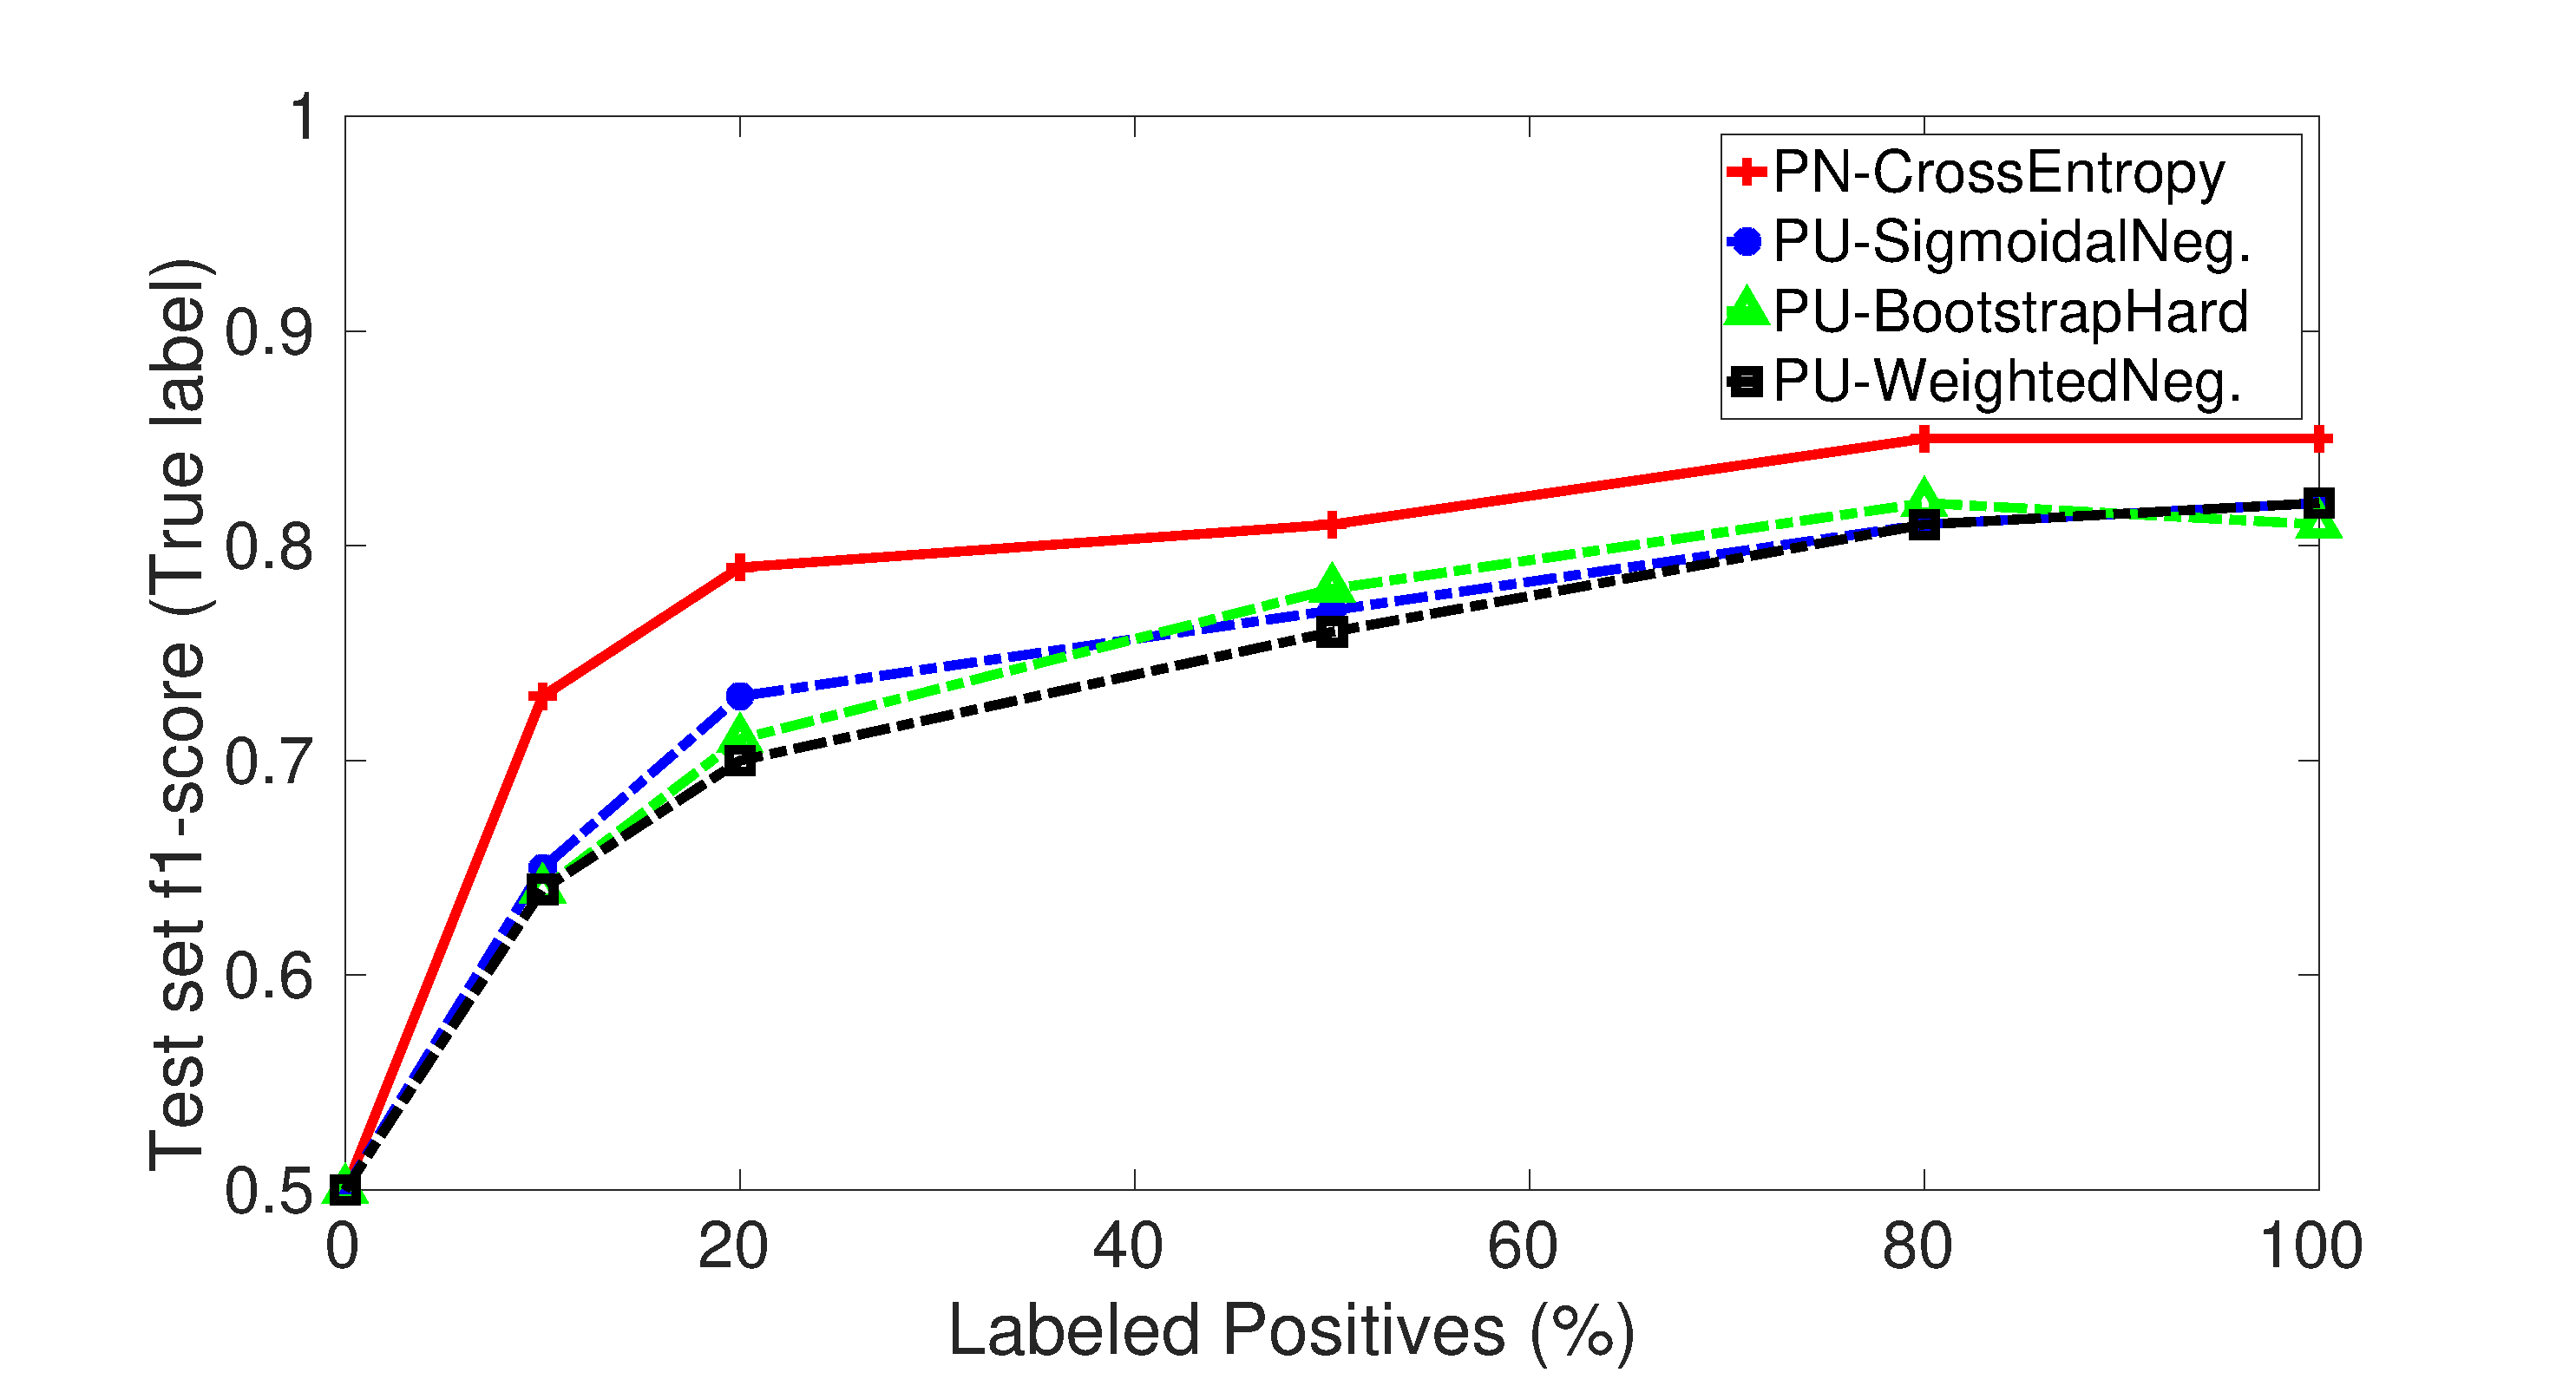
\includegraphics[width=\linewidth]{img/pu_vs_pn}
\caption{Varying percentage of labeled positive images. \textbf{P+N} represents training with percetage of images with reliable positive and negative labels and \textbf{P+U} stands for training with the positive (P) and unlabeled (U) sets.}
\label{fig:pct_annotating}
\end{figure}

%%%%%%%% Text Segmentation Pascal VOC2011
\noindent
In the segmentation setup, we used again the PASCAL VOC2011 dataset with extra segmentation\cite{hariharan2011semantic}.
We synthesized inexhaustive segmentations the same way as described in Section \ref{subsec:robustness}.
The same AlexNet-FCN model were trained together with the different loss functions for class 0 to predict binary segmentation, determining whether a pixel is correspondent to an object or not.
Only single-object images were used for training and testing in order to avoid the influence of two adjacent objects joining as one object because of  binary segmentation.
The same hyperparameters for optimization were used as in Section \ref{subsec:robustness}.
The trained models were evaluated with the test set of PASACAL VOC2011 segmentation dataset with binary segmentations.

\noindent
As shown in Table \ref{tab:pusegment}, the exponential unlabeled loss achieved the highest mean accuracy and a slightly lower overall accuracy.
In contrast to the improvement of mean accuracy, mean IU for models trained with either weighted unlabeled loss or exponential unlabeled loss did not show significant improvement to the normal cross entropy loss.


%%%%%%%% TABLE Segmentation Pascal VOC2011
\begin{table}[t]
\resizebox{\columnwidth}{!}{
\centering
\begin{tabular}{ll|llll}
Annotation  & Loss & overall acc. & mean acc. & f.w. IU & mean IU \\
\hline
% Complete            & CrossEnt.U       &  0.88 & 0.60 & 0.48 & 0.80 \\
% 50\%Unsegmented     & CrossEnt.U       &  0.83 & 0.31 & 0.27 & 0.70 \\
% 50\%Unsegmented     & WeightedU        &  0.83 & 0.34 & 0.29 & 0.70 \\
% 50\%Unsegmented     & ExponentialU     &  0.83 & 0.34 & 0.29 & 0.70 \\
Complete       & CrossEnt.U       &  0.90 & 0.85 & 0.82 & 0.75 \\
50\%Unseg.     & CrossEnt.U       &  0.85 & 0.68 & 0.73 & 0.60 \\
50\%Unseg.     & WeightedU        &  0.84 & 0.71 & 0.73 & \textbf{0.62} \\
50\%Unseg.     & ExponentialU     &  0.83 & \textbf{0.75} & 0.72 & \textbf{0.62} \\
\end{tabular}
}
\caption{
Best binary segmentation performance achieved on the test set of PASCAL VOC2011 segmentation dataset in the presence of inexhaustive segmentation.
Class weight 0.7:1.75 was used to balance the sample frequency difference of the two classes and negative loss were further weighted by a factor of 0.5 for weighted unlabeled loss.
Mean accuracy is equivalent to mean recall over classes.
Mean IU is the average intersection over union ratio (IU) over two classes and f.w. IU is the frequency weighted average of IU over the two classes.
Experiments were repeated twice and standard deviations were approximately 0.01.
}
\label{tab:pusegment}
\end{table}


%%%%%%%% Figure Segmentation Pascawl VOC2011
\noindent
Selective predictions for models trained with exponential unlabeled (ExpU.) loss and normal cross entropy (CrossEnt.) loss were presented in Figure \ref{fig:pusegment}.
For these two example images, the model trained with cross entropy loss failed to segment objects from images whereas exponential unlabeled loss segmented on the position of the objects though with coarse outlines.
The third column shows predictions given by model trained with complete training segmentation, and it did not give more accurate outlines.
The coarse results were mainly due to the limited compacity of AlexNet model.

\begin{figure}
\centering
  \begin{minipage}{\columnwidth}\footnotesize
  \centering
  \subsubfloat{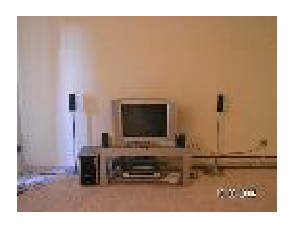
\includegraphics[width=0.19\columnwidth]{img/2007_002132}}{Raw}
  \subsubfloat{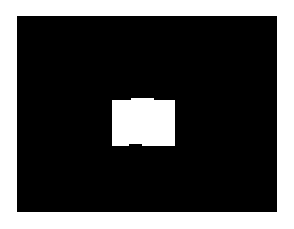
\includegraphics[width=0.19\columnwidth]{img/2007_002132_label}}{Label}
  \subsubfloat{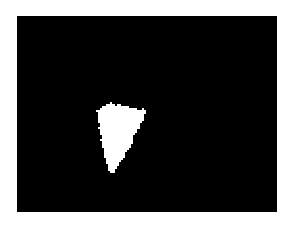
\includegraphics[width=0.19\columnwidth]{img/2007_002132_up_pred}}{Complete}
  \subsubfloat{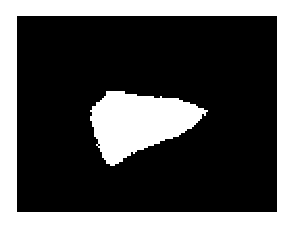
\includegraphics[width=0.19\columnwidth]{img/2007_002132_exp_pred}}{ExpU.}
  \subsubfloat{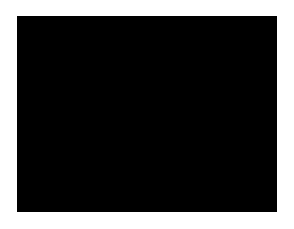
\includegraphics[width=0.19\columnwidth]{img/2007_002132_low_pred}}{CrossEnt.}
  \subsubfloat{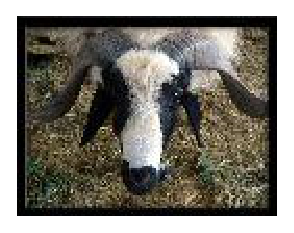
\includegraphics[width=0.19\columnwidth]{img/2007_002618}}{Raw}%
  \subsubfloat{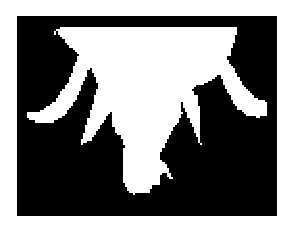
\includegraphics[width=0.19\columnwidth]{img/2007_002618_label}}{Label}
  \subsubfloat{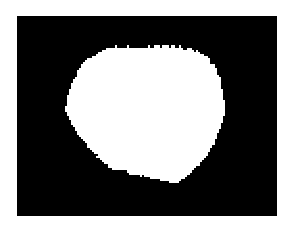
\includegraphics[width=0.19\columnwidth]{img/2007_002618_up_pred}}{Complete}
  \subsubfloat{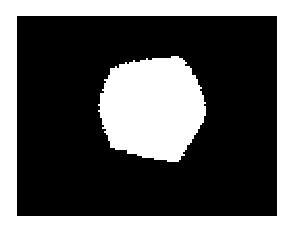
\includegraphics[width=0.19\columnwidth]{img/2007_002618_exp_pred}}{ExpU.}
  \subsubfloat{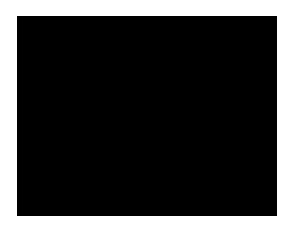
\includegraphics[width=0.19\columnwidth]{img/2007_002618_low_pred}}{CrossEnt.}
  \end{minipage}
\caption{Selective predictions for models in Table \ref{tab:pusegment}.}
\label{fig:pusegment}
\end{figure}


%%%%%%%% Text Fine-tuning performance with exponential loss
\noindent \textit{Exponential loss help improve fine-tuning performance}
Additionally,
